\chapter{The LHC and CMS experiment}
\label{sec:cms}

This chapter will explain the apparatus used to generate and collect the datasets that are utilised for the physics analysed described in Chapters~\ref{sec:bsm_H_to_tau_tau_analysis} and \ref{sec:H_A_to_4_tau_analysis}.
This is split into two parts.
Firstly, an overview of the \ac{LHC} and a description of how proton-proton collisions at a centre-of-mass energy ($\sqrt{s}$) of 13 TeV are achieved.
Secondly, an explanation of the \ac{CMS} detector is given, including a look at the individual sub-detectors, that are crucial to the reconstruction of particles originating from the proton-proton collisions.

\section{The LHC}

The \ac{LHC}~\cite{Evans:2008zzb}, located at \ac{CERN} just outside Geneva, is a synchrotron measuring 27 km in circumference, installed in the tunnel previously used by the \ac{LEP} accelerator \cite{203828}. 
Upon design, its primary purpose was to provide collisions between proton beams, generating centre-of-mass energies of up to 14 TeV and an instantaneous luminosity of approximately $10^{34}$ cm$^{−2}$s$^{−1}$. 
Figure~\ref{fig:CERN_Schematic} illustrates the arrangement of the \ac{LHC} and the \ac{CERN} accelerator complex. 
Protons are supplied to the \ac{LHC} through a sequence of accelerators: Linac4 (Linac2 pre-2020), \ac{PSB}, \ac{PS}, and the \ac{SPS}, that successively raise the energies of the protons to 50 MeV, 1.4 GeV, 25 GeV, and 450 GeV respectively. 
When the final energy has been achieved, the \ac{SPS} injects bunched protons into the \ac{LHC}'s beam pipes as two counter-rotating beams. 
Each bunch contains over $10^{11}$ protons, with each one separated by 25 ns and each beam consists of 2808 bunches. 
The protons are accelerated to collision energy using eight 400 MHz \ac{RF} cavities and kept in a circular trajectory with 1232 niobium-titanium superconducting dipole magnets. 
These magnets must be maintained at their operating temperature of 1.9 K to generate magnetic fields up to 8.4 T, requiring the use of superfluid helium. 
The bunches are collided at four intersection points surrounded by the ALICE~\cite{ALICE:2008ngc}, ATLAS~\cite{ATLAS:2008xda}, CMS~\cite{CMS_Setup} and LHCb~\cite{LHCb:2008vvz} detectors, at a collision rate of 40 MHz. \\

\begin{figure}[t]
    \centering
    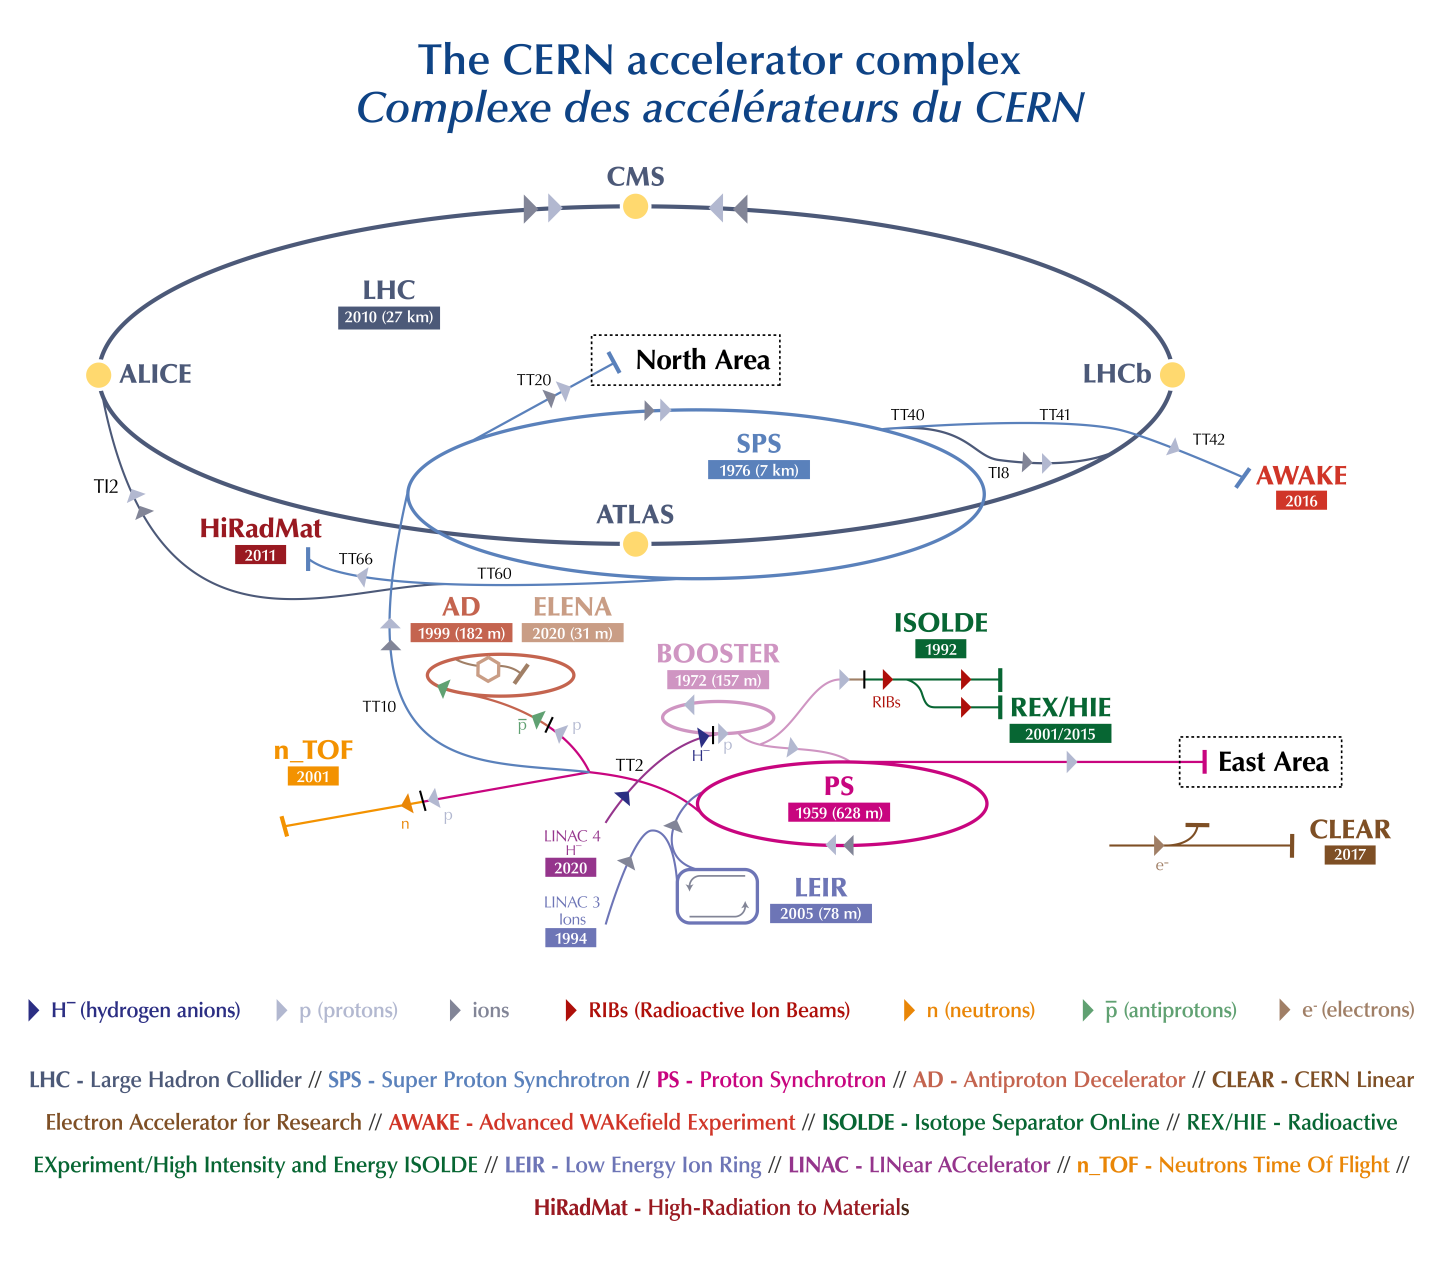
\includegraphics[width=\textwidth]{Figures/cern.png}
    \caption{A schematic diagram of the CERN accelerator complex~\cite{Bartosik:2847538}.}
    \label{fig:CERN_Schematic}
\end{figure}

The rate of events for a process produced in \ac{LHC} collisions can be expressed as,

\begin{equation}
R_{\text{event}} = L_{\text{inst}} \sigma(\sqrt{s}), 
\end{equation}

where $\sigma$ represents the cross-section of the process and is a function of the centre-of-mass energy, and $L_{\text{inst}}$ denotes the \ac{LHC} machine's instantaneous luminosity, that depends only on the beam parameters and can be calculated by,

\begin{equation}
L_{\text{inst}} = \frac{n_{b}N_{b}^{2}f_{\text{rev}}\gamma_{r}}{4\pi \epsilon_{n}\beta^{*}}F,
\end{equation}

where $n_b$ is the number of bunches per beam, $N_b$ is the number of particles per bunch, $f_{\text{rev}}$ is the revolution frequency, $\gamma_r$ is the relativistic gamma factor, $\epsilon_n$ is the normalised transverse beam emittance, $\beta^*$ is the beta function at the collision point, and $F$ is a reduction factor which accounts for the crossing angle of the beams at the collision point. 
One disadvantage of an increase in the instantaneous luminosity is the increase of \ac{PU}, defined as the number of additional inelastic proton-proton collisions per bunch crossing.

\begin{figure}[h]
    \centering
    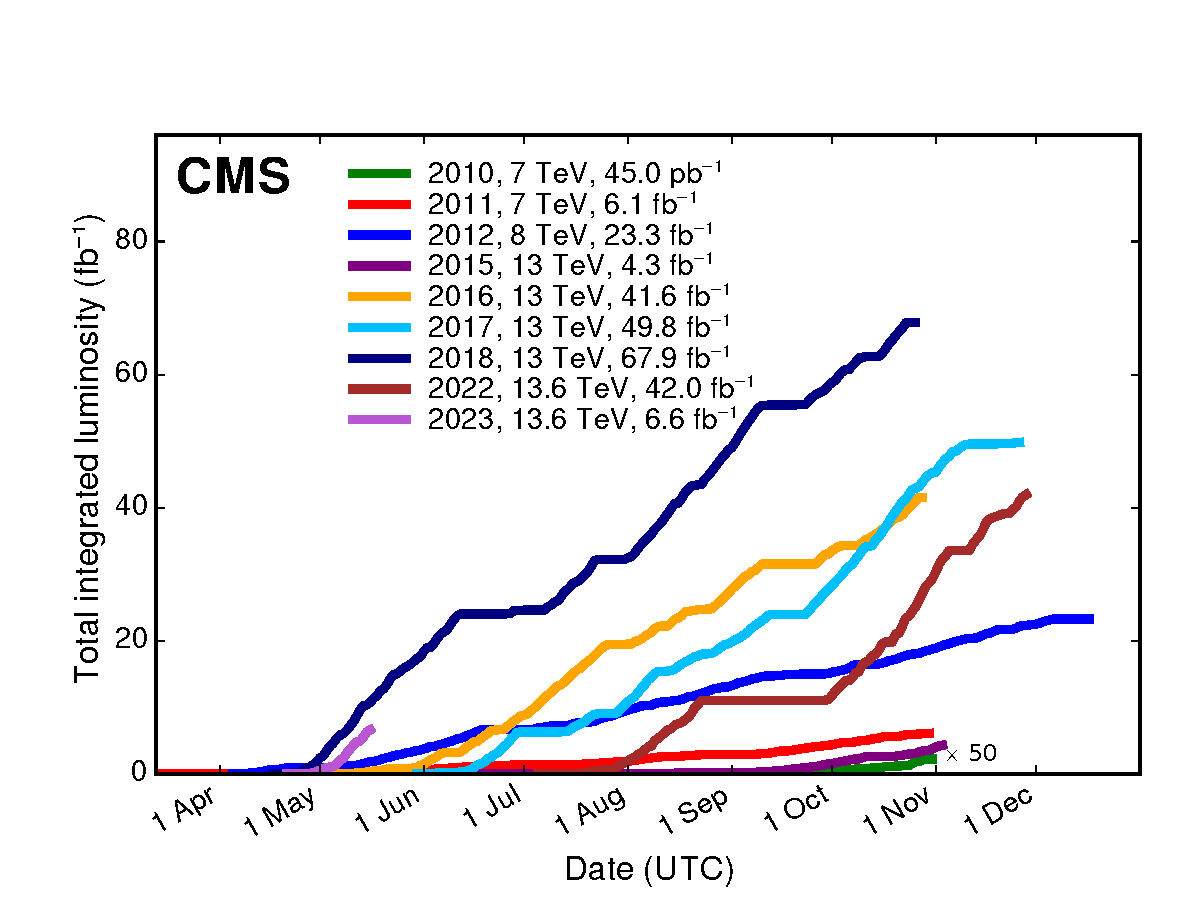
\includegraphics[width=0.9\textwidth]{Figures/int_lumi_cumulative_pp_2.pdf}
    \caption{The total integrated luminosity for proton-proton collisions collected by the \ac{CMS} experiment between 2010 and May 2023~\cite{lumi}.}
    \label{fig:int_lumi}
\end{figure}

The \ac{LHC} began its first physics collisions in 2010, initially colliding beams at $\sqrt{s}$ = 7 TeV, which was increased to 8 TeV throughout 2012. 
Following this data-taking period, known as Run 1, the \ac{LHC} underwent a two-year \ac{LS1} to undergo upgrades in preparation for an increase in $\sqrt{s}$. 
In 2015, the \ac{LHC} was restarted, initiating its Run 2 phase of data collection at $\sqrt{s}$ = 13 TeV, which lasted until the end of 2018. 
During Run 2, the \ac{LHC} achieved and surpassed its original design luminosity by obtaining a record peak luminosity of $2.1\times10^{34}$ cm$^{−2}$s$^{−1}$ in 2018.
Subsequently, the \ac{LHC} performed a second update period, the \ac{LS2}, lasting for approximately three years, whereafter the data collection for Run 3 began at $\sqrt{s}$ = 13.6 TeV.
Figure~\ref{fig:int_lumi} illustrates the total integrated luminosity of proton-proton collisions delivered to the \ac{CMS} detector at the time of writing.
The data used for the analyses described in this thesis correspond to the full Run 2 dataset collected during the 2016--2018 data-taking periods at 13 TeV. 
Only data recorded by \ac{CMS}, where all sub-detectors were functioning correctly, are certified for use in physics analyses. 
This equates to 36.3 fb$^{−1}$, 41.5 fb$^{−1}$ and 59.7 fb$^{-1}$ of data collected in 2016, 2017 and 2018 respectively. \\

\section{The CMS detector}

The \ac{CMS} detector was engineered to fulfil the rigorous demands of the \ac{LHC} physics program. 
Its primary objective is to achieve sensitivity to the Higgs boson and novel phenomena at the TeV energy scale. 
Weighing 12,500 tonnes and measuring 21.6 m in length with a diameter of 14.6 m, the \ac{CMS} detector uses an array of sub-detectors encircling the central beam axis. 
The layout of the \ac{CMS} detector is shown in Figure~\ref{fig:CMS_Schematic}.
A superconducting solenoid, operating at a magnetic field strength of 3.8 T, surrounds the inner tracker, electromagnetic calorimeter, and hadronic calorimeter. 
Situated outside the solenoid within the iron return yoke are gaseous muon detectors, positioned to accurately measure muons. 
The \ac{CMS} detector adopts a coordinate system centred at the collision point, with the $y$-axis oriented vertically, the $x$-axis directed radially inward toward the \ac{LHC} centre, and the $z$-axis aligned with the beam direction. 
The transverse energy ($E_T$) and transverse momentum ($\pT$) are defined in the $x$-$y$ plane. 
The azimuthal angle ($\phi$) and polar angle ($\theta$) are measured relative to the $x$-axis in the $x$-$y$ plane and $z$-axis relative to the $z$-$y$ plane, respectively. 
$r$ is used as the radial distance in the $x$-$y$ plane.
Pseudorapidity ($\eta$), defined as $\eta = -\ln[\tan(\theta/2)]$, is used due to its gauge invariance, and distances between objects in the $\phi$-$\eta$ plane are characterised by the metric $\Delta R = \sqrt{\Delta\phi^2 + \Delta\eta^2}$. 

\begin{figure}[h]
    \centering
    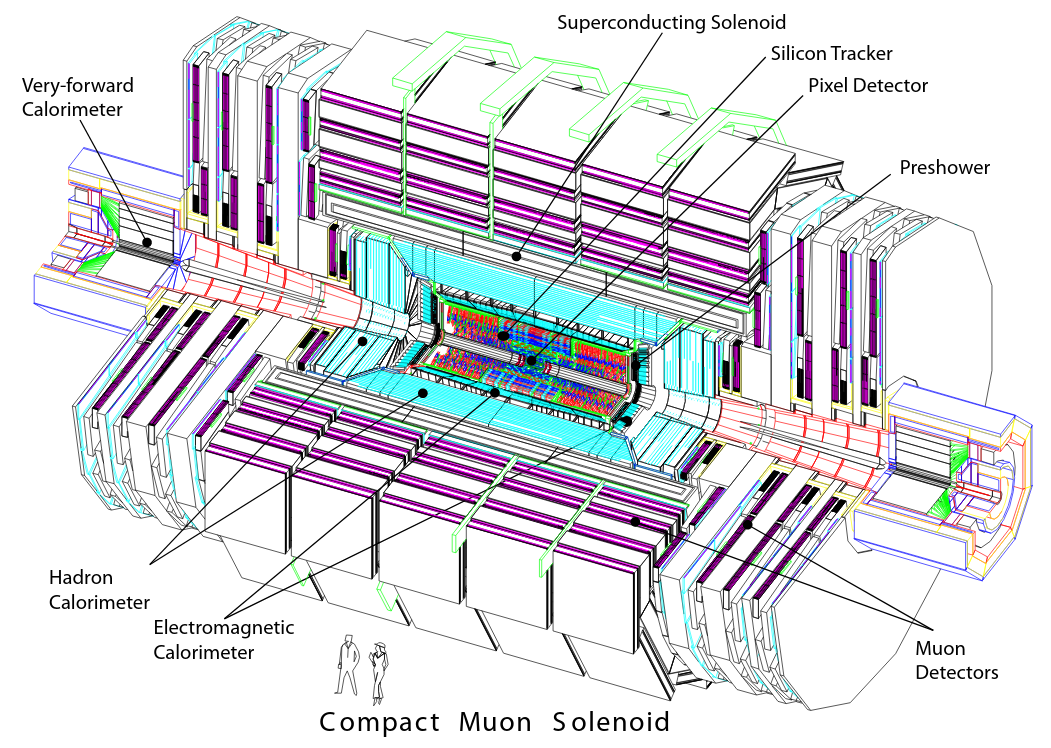
\includegraphics[width=0.9\textwidth]{Figures/CMS_Detector.png}
    \caption{A perspective view of the \ac{CMS} detector \cite{CMS_Setup}.}
    \label{fig:CMS_Schematic}
\end{figure}

\subsection{Tracker}

Closest to the interaction point in the \ac{CMS} experiment is the tracker~\cite{CMS_Setup,Malberti:2014pda,CMS:2012sda}, which is essential for precise measurements of charged particle trajectories and the determination of the \ac{PV} and other vertices, as explained in Section~\ref{sec:track_and_vertex}. 
To meet the requirements of high granularity and fast response for the large number of particles generated in each bunch crossing, as well as being radiation hard to deal with the particle flux, a silicon tracking detector is utilised. 
The tracker consists of a pixel detector and a silicon strip detector as shown in Figure~\ref{fig:tracker}. \\

\begin{figure}[!hbtp]
    \centering
    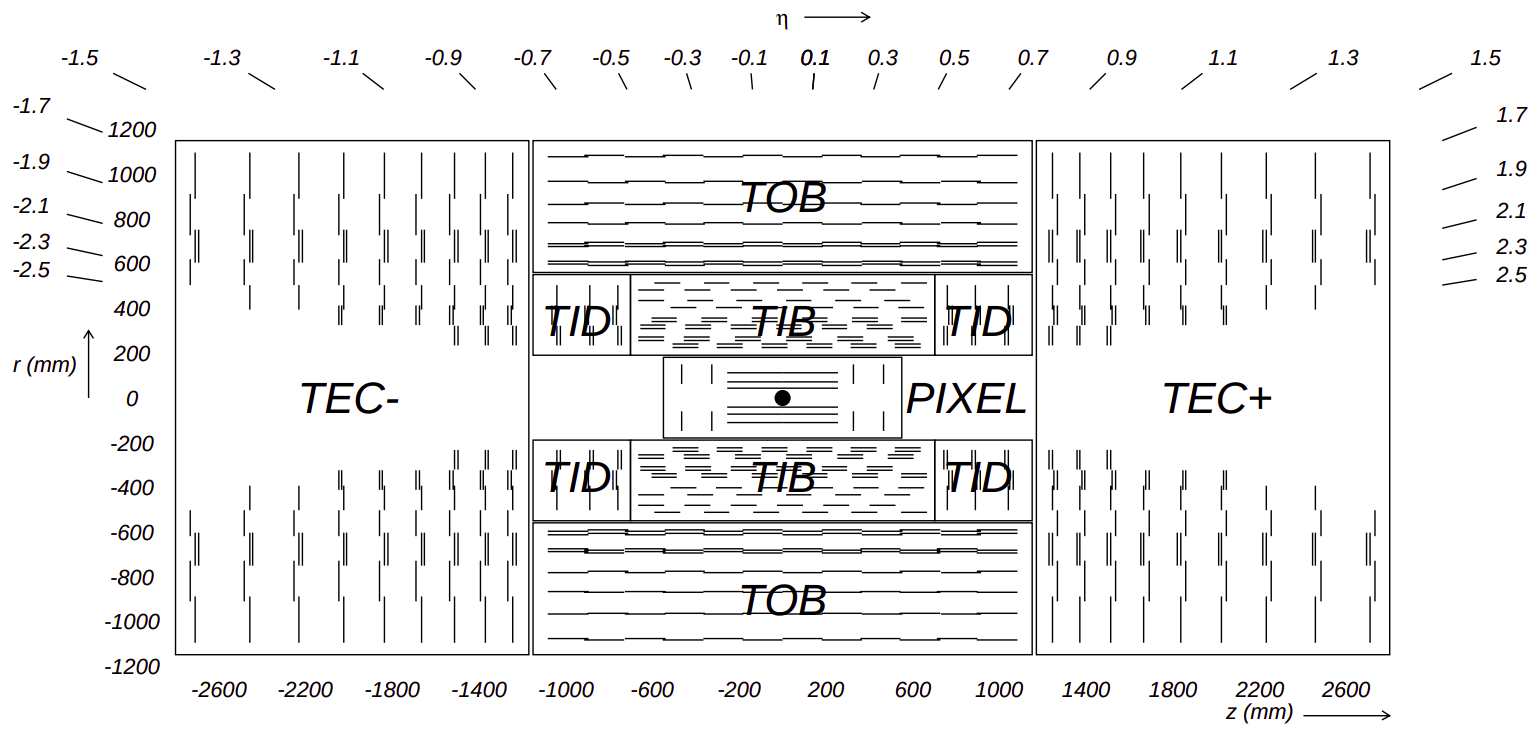
\includegraphics[width=\textwidth]{Figures/tracker.png}
    \caption{Schematic of the CMS tracker (pre-pixel upgrade) in the $r$-$z$ plane, showing the position of the pixel detector as well as the TIB, TID, TOB, and TEC strip detectors. The lines represent detector modules and the double lines represent back-to-back modules~\cite{CMS_Setup}.}
    \label{fig:tracker}
\end{figure}

The pixel detector covers the pseudorapidity range $|\eta| < 2.5$ and is composed of three cylindrical pixel modules and two disk pixel modules. 
It contains 66 million silicon pixels, each with dimensions of $100 \times 150$ $\upmu$m${^2}$. 
This configuration provides a spatial resolution of 15--20 $\upmu$m in both the $r$-$\phi$ plane and the $z$ direction, enabling three-dimensional vertex reconstruction.
The original tracker was built to handle an instantaneous luminosity of $10^{34}$ cm$^{2}$s$^{-1}$ and an average \ac{PU} of 25.
To handle higher luminosities and increased event \ac{PU}, the pixel detector was upgraded in 2016/2017 to handle approximately double the instantaneous luminosity and \ac{PU}~\cite{CMS:2012sda}. 
The upgraded detector consists of four barrel module layers and three endcap disks, resulting in 124 million pixels. \\

Surrounding the pixel detector is the silicon strip detector, which is divided into four subsystems: the \ac{TIB}, \ac{TID}, \ac{TOB}, and \ac{TEC}. 
The \ac{TIB} and \ac{TID} provide four layers of silicon strip detectors in the barrel region and three disks at each end, extending up to a radius of 55 cm. 
The \ac{TOB} consists of six barrel layers extending up to an outer radius of 116 cm, while the \ac{TEC} comprises nine disks covering a range of $|z|$ from 124 cm to 282 cm. 
The silicon strips have various thicknesses and widths, providing multiple measurements of the $r$-$\phi$ position with resolutions ranging from 23-35 $\upmu$m in the \ac{TIB} to 35-53 $\upmu$m in the \ac{TOB}. \\

In addition to the main components, the tracker includes back-to-back mounted micro-strip detector modules to provide additional measurements of the $z$ coordinate in specific regions. 
The overall tracker layout ensures the presence of at least three hits in the pixel detector (at least four hits for the upgraded detector) and at least nine hits in the silicon-strip tracker, with a minimum of four two-dimensional measurements among them.

\subsection{Electromagnetic calorimeter}

The \ac{CMS} \ac{ECAL} is a hermetic homogeneous calorimeter designed to detect high-energy electrons and photons~\cite{CMS_Setup,CMS:2013lxn}. 
In total, 75,848 lead tungstate (PbWO$_4$) crystals are sorted in a barrel and endcap configuration. 
PbWO$_4$ was chosen as the crystal material due to its radiation hardness, high density, short radiation length, and small Molière radius (the average radius containing on average 90\% of
a shower’s total energy deposit), enabling the construction of a compact and finely granular \ac{ECAL}. 
Scintillation light produced by showering electrons and photons in the crystals is converted into an electrical signal by photodetectors such as avalanche photodiodes in the barrel and vacuum phototriodes in the endcaps. 
The scintillation decay time of the crystals matches the 25 ns \ac{LHC} bunch crossing time, ensuring that a significant portion of the light is emitted between bunch crossings. \\

The \ac{ECAL} is placed outside of the tracker but within the magnet bore and covers the pseudorapidity range $|\eta| < 3.0$. 
It comprises of an \ac{EB} covering $|\eta| < 1.479$ and an \ac{EE} covering $1.479 < |\eta| < 3.0$. 
A diagram of this is shown in Figure~\ref{fig:ecal}.
The barrel region consists of 61,200 crystals with 360-fold granularity in $\phi$ and 170-fold granularity in $\eta$. 
The crystals are tapered with a front face area of $0.0174 \times 0.0174$ in $\eta$-$\phi$ ($22 \times 22$ mm$^2$) and a length of 230 mm. 
The endcaps house 7,324 crystals arranged in a rectangular $x$-$y$ grid, each with a front face area of $28.62 \times 28.62$ mm$^2$ and a length of 220 mm. \\

The \ac{ECAL} system also includes pre-shower detectors placed in front of each endcap to identify photons from neutral pion decays and improve electron identification and position resolution. 
These detectors consist of lead radiators to initiate showering and silicon-strip sensors to measure the deposited energy. 
The \ac{ECAL} energy resolution is parametrised as a function of the incident particle energy E, with terms for the stochastic S, noise N, and constant C contributions.

\begin{equation}
\Big(\frac{\sigma}{E}\Big)^2 = \Big(\frac{S}{\sqrt{E}}\Big)^2 + \Big( \frac{N}{E} \Big) + C^2
\end{equation}

The stochastic term captures fluctuations in lateral shower containment and photon yield, the noise term accounts for electronics' noise and \ac{PU}, and the constant term arises from the non-uniformity of the longitudinal response and calibration errors. 
Measurements using electron beams have determined the values of S = 0.028 GeV$^{1/2}$, N = 0.12 GeV, and C = 0.003 for the \ac{ECAL} energy resolution.

\begin{figure}[!hbtp]
    \centering
    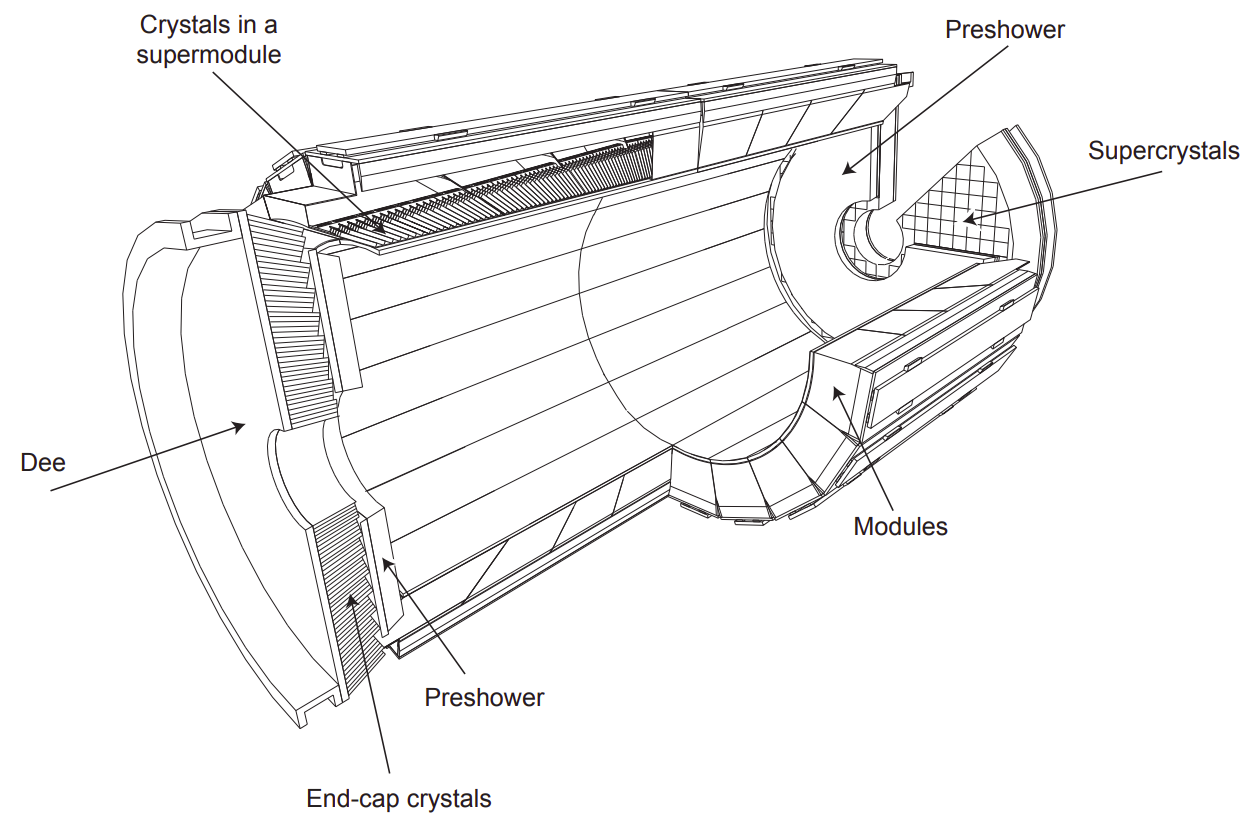
\includegraphics[width=\textwidth]{Figures/ECAL.png}
    \caption{A schematic of the CMS ECAL detector~\cite{CMS_Setup}.}
    \label{fig:ecal}
\end{figure}

\subsection{Hadronic calorimeter}

The \ac{CMS} detector includes the \ac{HCAL}, which plays a crucial role in measuring the energies of strongly interacting particles and being able to reconstruct missing energy signals. 
The \ac{HCAL} is located outside of the \ac{ECAL} and covers the pseudorapidity region $|\eta| < 5.2$. 
It consists of four sub-detectors: the \ac{HB}, \ac{HE}, \ac{HO}, and \ac{HF} calorimeters, arranged as shown in Figure~\ref{fig:hcal}.

\begin{figure}[!hbtp]
    \centering
    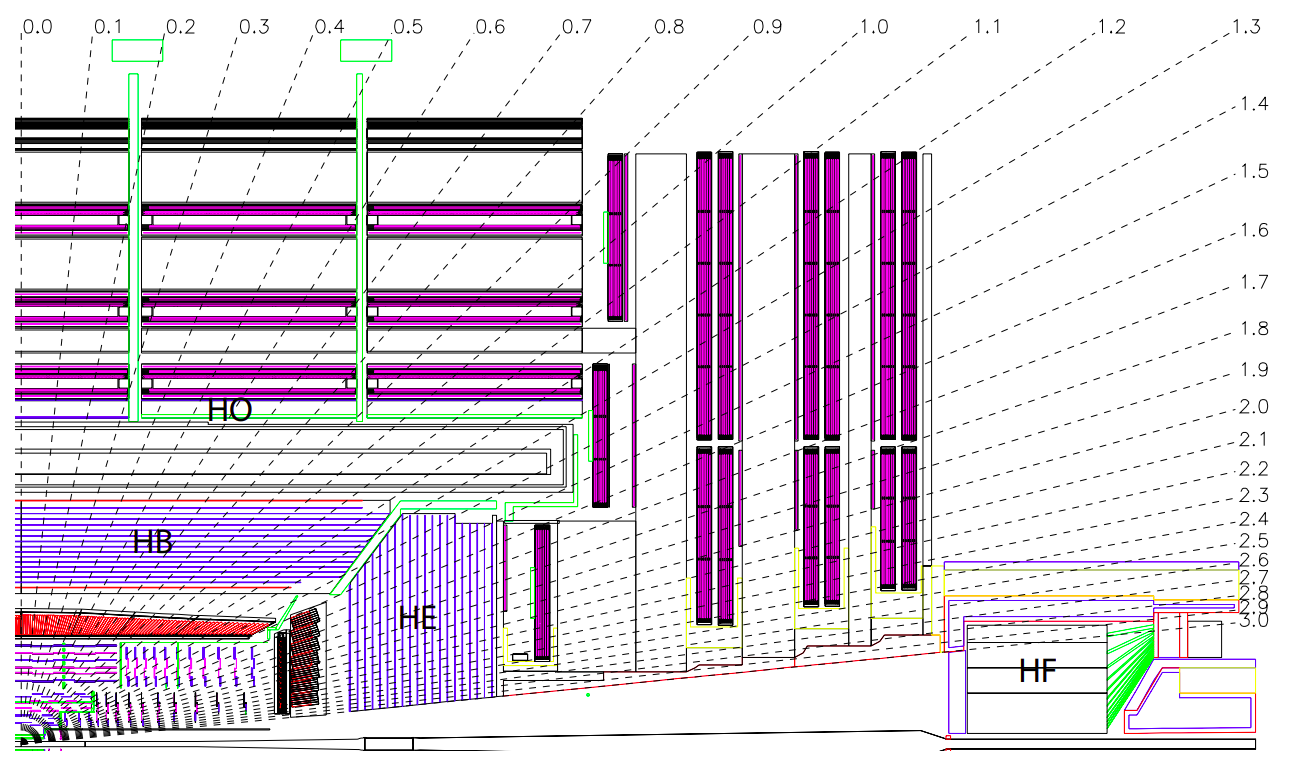
\includegraphics[width=\textwidth]{Figures/HCAL.png}
    \caption{A schematic of the CMS HCAL showing the arrangement of the HB, HE, HO, and HF calorimeters. The numbers represent the $|\eta|$ value in the detector~\cite{CMS_Setup}.}
    \label{fig:hcal}
\end{figure}

The \ac{HB} and \ac{HE} calorimeters are positioned within the magnet bore, covering the pseudorapidity regions $|\eta| < 1.3$ and $1.3 < |\eta| < 3.0$, respectively. 
They are constructed using alternating layers of brass absorber plates and plastic scintillator tiles. 
Brass is chosen as the absorber material due to its short nuclear interaction length and non-magnetic properties. 
The \ac{HB} provides 5.82 to 10.6 interaction lengths of absorber material, while the \ac{HE} provides approximately 10 interaction lengths. 
The plastic scintillator tiles collect scintillation light emitted by charged particles in the hadronic showers, which is then read out using hybrid photodiodes. \\

To extend the \ac{HCAL}'s containment capability in the central detector region ($|\eta| < 1.3$), the \ac{HO} calorimeter is utilised. 
It is placed outside of the solenoid coil and utilises plastic scintillator tiles as the active material. 
The \ac{HO} enhances the thickness of the \ac{HCAL} to a minimum of 11.8 interaction lengths, improving the measurement of late-starting or highly penetrating showers. \\

In the forward regions ($|\eta| > 3.0$), the \ac{HF} detector extends the pseudorapidity coverage of the \ac{HCAL} up to $|\eta| < 5.2$. 
The \ac{HF} is subjected to a high flux of incoming particles, and therefore, requires extremely radiation-hard materials. 
Quartz fibres embedded in steel absorbers are employed as the active material. Charged particles in the showers generate Cherenkov light in the quartz fibres, which is detected by photomultiplier tubes. \\

The energy resolution of the \ac{HCAL} can be parametrised as a function of the incident particle energy E, using the formula, 
\begin{equation}
\Big(\frac{\sigma}{E}\Big)^2 = \Big(\frac{S}{\sqrt{E}}\Big)^2 + C^2
\end{equation}

where the stochastic term S is measured to be 0.943 GeV${^{1/2}}$ and the constant term C is measured to be 0.084.
During the \ac{LS1} period, upgrades were performed on the photomultiplier tubes of the \ac{HF}.

\subsection{Muon system}

The muon system in the \ac{CMS} detector plays a crucial role in the accurate identification and measurement of muons, which are essential for various physics analyses. 
The system is designed with three primary functions: efficient muon identification, precise momentum measurement, and triggering capability. \\

Located outside the solenoid coil and \ac{HO} calorimeter, the muon system is strategically positioned between the iron plates forming the flux return yoke. 
This arrangement takes advantage of the high-field solenoidal magnet and the yoke's structure to enable the desired functions.
The muon system covers a wide pseudorapidity range, specifically $|\eta| < 2.4$. 
It consists of three types of gaseous detectors: \ac{DT} chambers, \ac{CSC}, and \ac{RPC}. \\

In the region of $|\eta| < 1.2$, the muon system employs \ac{DT} chambers, which are organised into four stations. 
These include inner and outer stations positioned inside and outside the magnet return yoke, as well as two stations inter-spaced between the iron layers of the yoke. 
The \ac{DT} chambers are composed of rectangular drift cells filled with a mixture of argon and carbon dioxide gas. 
Each cell features an anode wire running along its length. 
The cells are arranged into superlayers, each containing four layers of cells. 
The \ac{DT} chambers in the three innermost muon stations consist of three superlayers, whereas the outer station contains only two superlayers. 
The spatial resolution of the \ac{DT} chambers is measured to be 77–123 $\upmu$m for the $\phi$ coordinate measurement and 133–393 $\upmu$m for the $z$ coordinate measurement. \\

In the region of $0.9 < |\eta| < 2.4$, the \ac{CSC}s are employed. 
These chambers are trapezoidal-shaped multiwire proportional chambers with six layers of gas. 
The gas mixture used includes argon, carbon dioxide, and tetrafluoromethane. 
The \ac{CSC} modules are organised into four stations positioned between the endcap layers of the magnet's return yoke. 
They consist of layers of cathode strips and anode wires, allowing for measurements of the muon's $\phi$ and $r$ coordinates, respectively. 
The spatial resolution per chamber of the \ac{CSC}s ranges from 45 $\upmu$m to 143 $\upmu$m. \\

To enhance the system's capabilities in the $|\eta| < 1.6$ region, \ac{RPC}s are used. 
These parallel-plate detectors feature a double-gap module design with anode and cathode plates separated by a gas gap. 
The \ac{RPC}s are embedded within the barrel and endcap iron yokes. 
In the barrel, six layers of \ac{RPC} chambers are present, with two layers in each of the two innermost muon stations and one layer in each of the two outer stations. 
In the endcap, the \ac{RPC}s consist of four layers positioned on either side of the three iron disks. 
While the \ac{RPC}s exhibit a lower spatial resolution compared to the \ac{DT}s and \ac{CSC}s (0.78–1.38 cm per chamber), they offer a remarkably fast response time, making them suitable for dedicated muon triggering.

\subsection{Triggering and computing}

The \ac{LHC} collides protons at a rate of 40 MHz during its operation. 
However, it is impractical to read out and store every event due to the high data volume involved. 
To address this challenge, the \ac{CMS} detector employs a dedicated trigger system that selectively chooses the most interesting events, reducing the recorded rate to around 1 kHz. \\

The \ac{CMS} trigger system consists of two stages: the \ac{L1} trigger and the \ac{HLT}. 
The \ac{L1} trigger, implemented with custom-built programmable electronics, operates as the first stage and reduces the event rate to approximately 100 kHz. 
During the upgrade in 2015/2016, the \ac{L1} system was enhanced to accommodate the increased instantaneous luminosity and \ac{PU} conditions. 
Upgrades included improved muon momentum resolution, electron/photon isolation, hadronic tau identification and isolation, jet-finding algorithms with \ac{PU} subtraction, and enhanced trigger menu capabilities. \\

The \ac{L1} trigger utilises a time multiplexed architecture, where energy deposits recorded in the calorimeters and hits from the muon detectors are processed. 
In the calorimeter trigger, energy deposits from the \ac{HCAL} and \ac{ECAL} are passed through two layers (Layer 1 and Layer 2), enabling object identification and the selection of the best candidates based on their $\pT$. 
Simultaneously, hits from the muon detectors are combined in the muon trigger's tracking finder and sorting/merging layers, producing a sorted list of muon candidates for the entire detector. 
The global trigger then integrates the information from both calorimeter and muon triggers to decide on event selection within a maximum storage time of 3.2 $\upmu$s.
A diagrammatic representation of this is shown in Figure~\ref{fig:trigger}. \\

\begin{figure}[!hbtp]
    \centering
    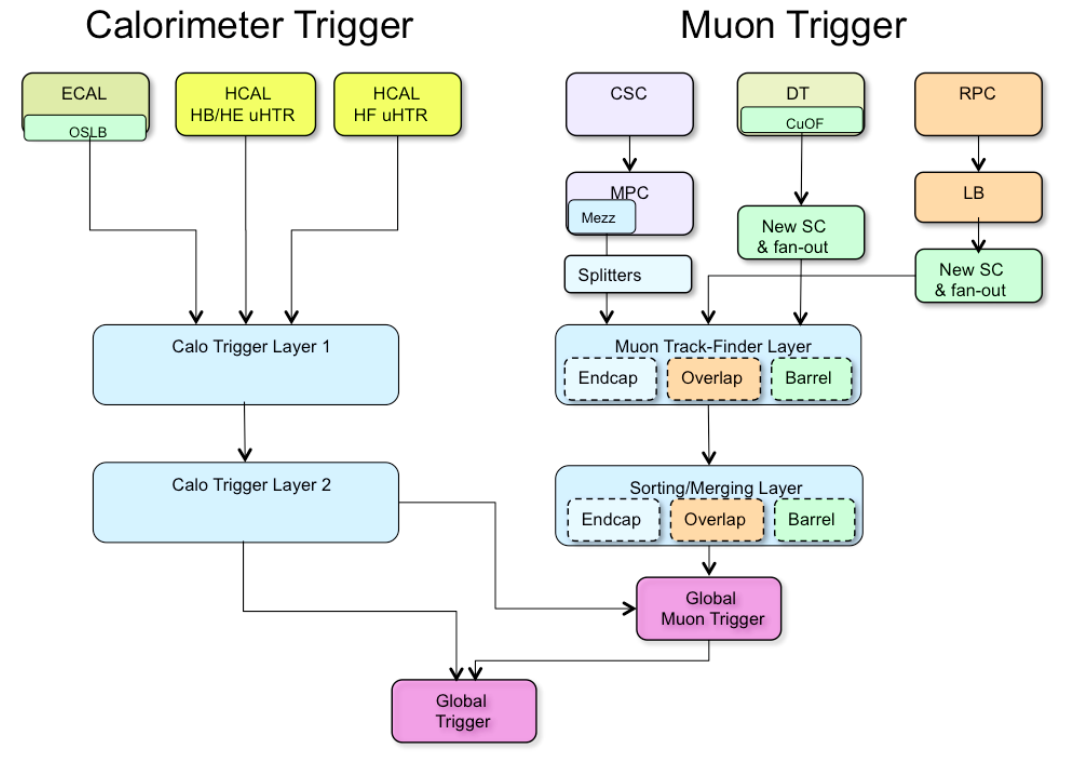
\includegraphics[width=\textwidth]{Figures/trigger.png}
    \caption{A schematic of the L1 trigger workflow for object reconstruction~\cite{Tapper:2013yva}.}
    \label{fig:trigger}
\end{figure}

The second stage of the trigger system is the \ac{HLT}, which is a software-based trigger running on a multi-processor farm with thousands of CPU cores. 
The \ac{HLT} utilises information from the full detector, including the tracker, calorimeters, and muon systems. 
By closely following the algorithms and selections used offline, the \ac{HLT} ensures good momentum resolution and high identification efficiencies for selected objects. 
From the initial event rate of approximately 100 kHz received from the \ac{L1} trigger, the \ac{HLT} further reduces the output rate to about 1 kHz. \\

The events selected by the \ac{HLT} produce a significant amount of data, approximately $\mathcal{O}$(10 pb) per year. 
To process, store, and facilitate easy access for analysts worldwide, \ac{CMS} collaborates with other \ac{LHC} experiments through the \ac{WLCG}. 
The \ac{WLCG} combines computing resources from research institutions globally, organised into three tiers. 
Tier-0 sites, comprising the \ac{CERN} Data Center and the Wigner Research Centre in Budapest, perform full data reconstruction and store a copy of the data on tape. 
The data is then distributed to Tier-1 centres, which handle the storage of raw, reconstructed, and simulated data, as well as the distribution to Tier-2 sites. 
Tier-2 sites, located at universities and research institutes worldwide, provide computing resources for data production, reconstruction, and analysis by researchers.
